% ============================================================
%  SZU Experiment Report Template
%  Produced by: Chao Fan and Kewei Ou, AI School of SZU
% ============================================================

\documentclass[a4paper,12pt]{article}

% ----------------------------
% Chinese font and page setup
% ----------------------------
\usepackage{fontspec}
\usepackage{xeCJK}
\IfFontExistsTF{Noto Serif CJK SC}
  {\setCJKmainfont{Noto Serif CJK SC}}
  {\setCJKmainfont{SimSun}}

\usepackage{geometry}
\geometry{left=1in, right=1in, top=1in, bottom=1in}

\usepackage{longtable}
\usepackage{booktabs}
\usepackage{array}
\usepackage{graphicx}
\usepackage{fancyhdr}
\usepackage{tikz}
\usetikzlibrary{arrows.meta,calc,fit,positioning,shapes.geometric}
\usepackage{verbatim}
\usepackage{float}
\usepackage{amsmath}
\usepackage{amssymb}
\usepackage{xcolor}
\usepackage{caption}
\usepackage{hyperref}
\hypersetup{hidelinks}
\urlstyle{same}

\definecolor{szured}{RGB}{190,30,45}
\definecolor{szuredlight}{RGB}{255,238,240}
\definecolor{ink}{RGB}{35,39,47}
\definecolor{muted}{RGB}{95,101,113}
\definecolor{lineblue}{RGB}{63,103,148}

\captionsetup{
  font=small,
  labelfont=bf,
  textfont=it,
  justification=raggedright,
  singlelinecheck=false,
  skip=6pt
}

\fancyhf{}
\fancyhead[C]{}
\fancyhead[R]{}

\setlength{\parindent}{0pt}
\setlength{\parskip}{0.5em}

% ============================================================
% Document
% ============================================================
\begin{document}

% ============================================================
% Cover page
% ============================================================
\begin{titlepage}
    \centering
    \vspace*{2cm}
    \Huge{\textbf{深 \ 圳 \ 大 \ 学 \ 实 \ 验 \ 报 \ 告}}\\[1.5cm]

    {\Large\textbf{课程名称}\quad\underline{\makebox[8cm][c]{Python程序设计}}}\\[0.5cm]
    {\Large
    \noindent\makebox[3.2cm][l]{\textbf{项目名称}}
    \underline{\makebox[8cm][c]{\normalsize 纯 NumPy 实现 OpenCLIP 图像编码器}}}\\[0.5cm]
    {\Large
    \noindent\makebox[3.2cm][l]{\textbf{学 \quad \quad 院}}
    \underline{\makebox[8cm][c]{人工智能学院}}}\\[0.5cm]
    {\Large
    \noindent\makebox[3.2cm][l]{\textbf{专 \quad \quad 业}}
    \underline{\makebox[8cm][c]{人工智能}}}\\[0.5cm]
    {\Large
    \noindent\makebox[3.2cm][l]{\textbf{指导教师}}
    \underline{\makebox[8cm][c]{舒婷}}}\\[0.5cm]
    {\Large
    \noindent\makebox[3.2cm][l]{\textbf{报 \quad 告 \quad 人}}
    \underline{\makebox[3cm][c]{}}
    \hspace{0.5cm}
    \textbf{学号}
    \underline{\makebox[3cm][c]{}}}\\[0.5cm]
    {\Large
    \noindent\makebox[3.2cm][l]{\textbf{实验时间}}
    \underline{\makebox[8cm][c]{}}}\\[0.5cm]
    {\Large
    \noindent\makebox[3.2cm][l]{\textbf{提交时间}}
    \underline{\makebox[8cm][c]{}}}\\[1.5cm]

    \vfill
    \Large{\textbf{教务处制}}
\end{titlepage}

\newpage

% ============================================================
% Main body
% ============================================================
\section{Objectives}

This project reconstructs the image tower of OpenCLIP ViT-B/32 as a
fixed-parameter forward computation implemented with NumPy. The objective is
not to train or fine-tune a model, but to reproduce the supplied checkpoint's
numerical behavior through explicit array operations.

The required interface accepts preprocessed RGB images with shape
\([B,3,224,224]\), extracts \(7\times 7\) image patches, processes the resulting
token sequence through twelve Transformer blocks, and returns one
L2-normalized 512-dimensional output token for each image. The implementation
must preserve \texttt{float32} precision and match the supplied stage-wise
references within the course tolerances.

\section{Overview}

The implementation follows the actual tensor flow of the image encoder. The
input image is divided into \(32\times32\) patches, projected into a 768-wide
feature space, combined with a learned CLS token and positional embeddings, and
then normalized. Twelve identical Transformer blocks repeatedly apply
multi-head self-attention, residual addition, an MLP, and a second residual
addition. The final CLS representation is normalized, projected from 768 to
512 dimensions, and L2-normalized row by row.

Figure~\ref{fig:vit-arch} summarizes the computation and uses red highlighting
to identify the six assessed implementation groups. The implementation uses
the supplied preprocessing and numerical helpers; model parameters remain
fixed throughout.

\begin{figure}[H]
\centering
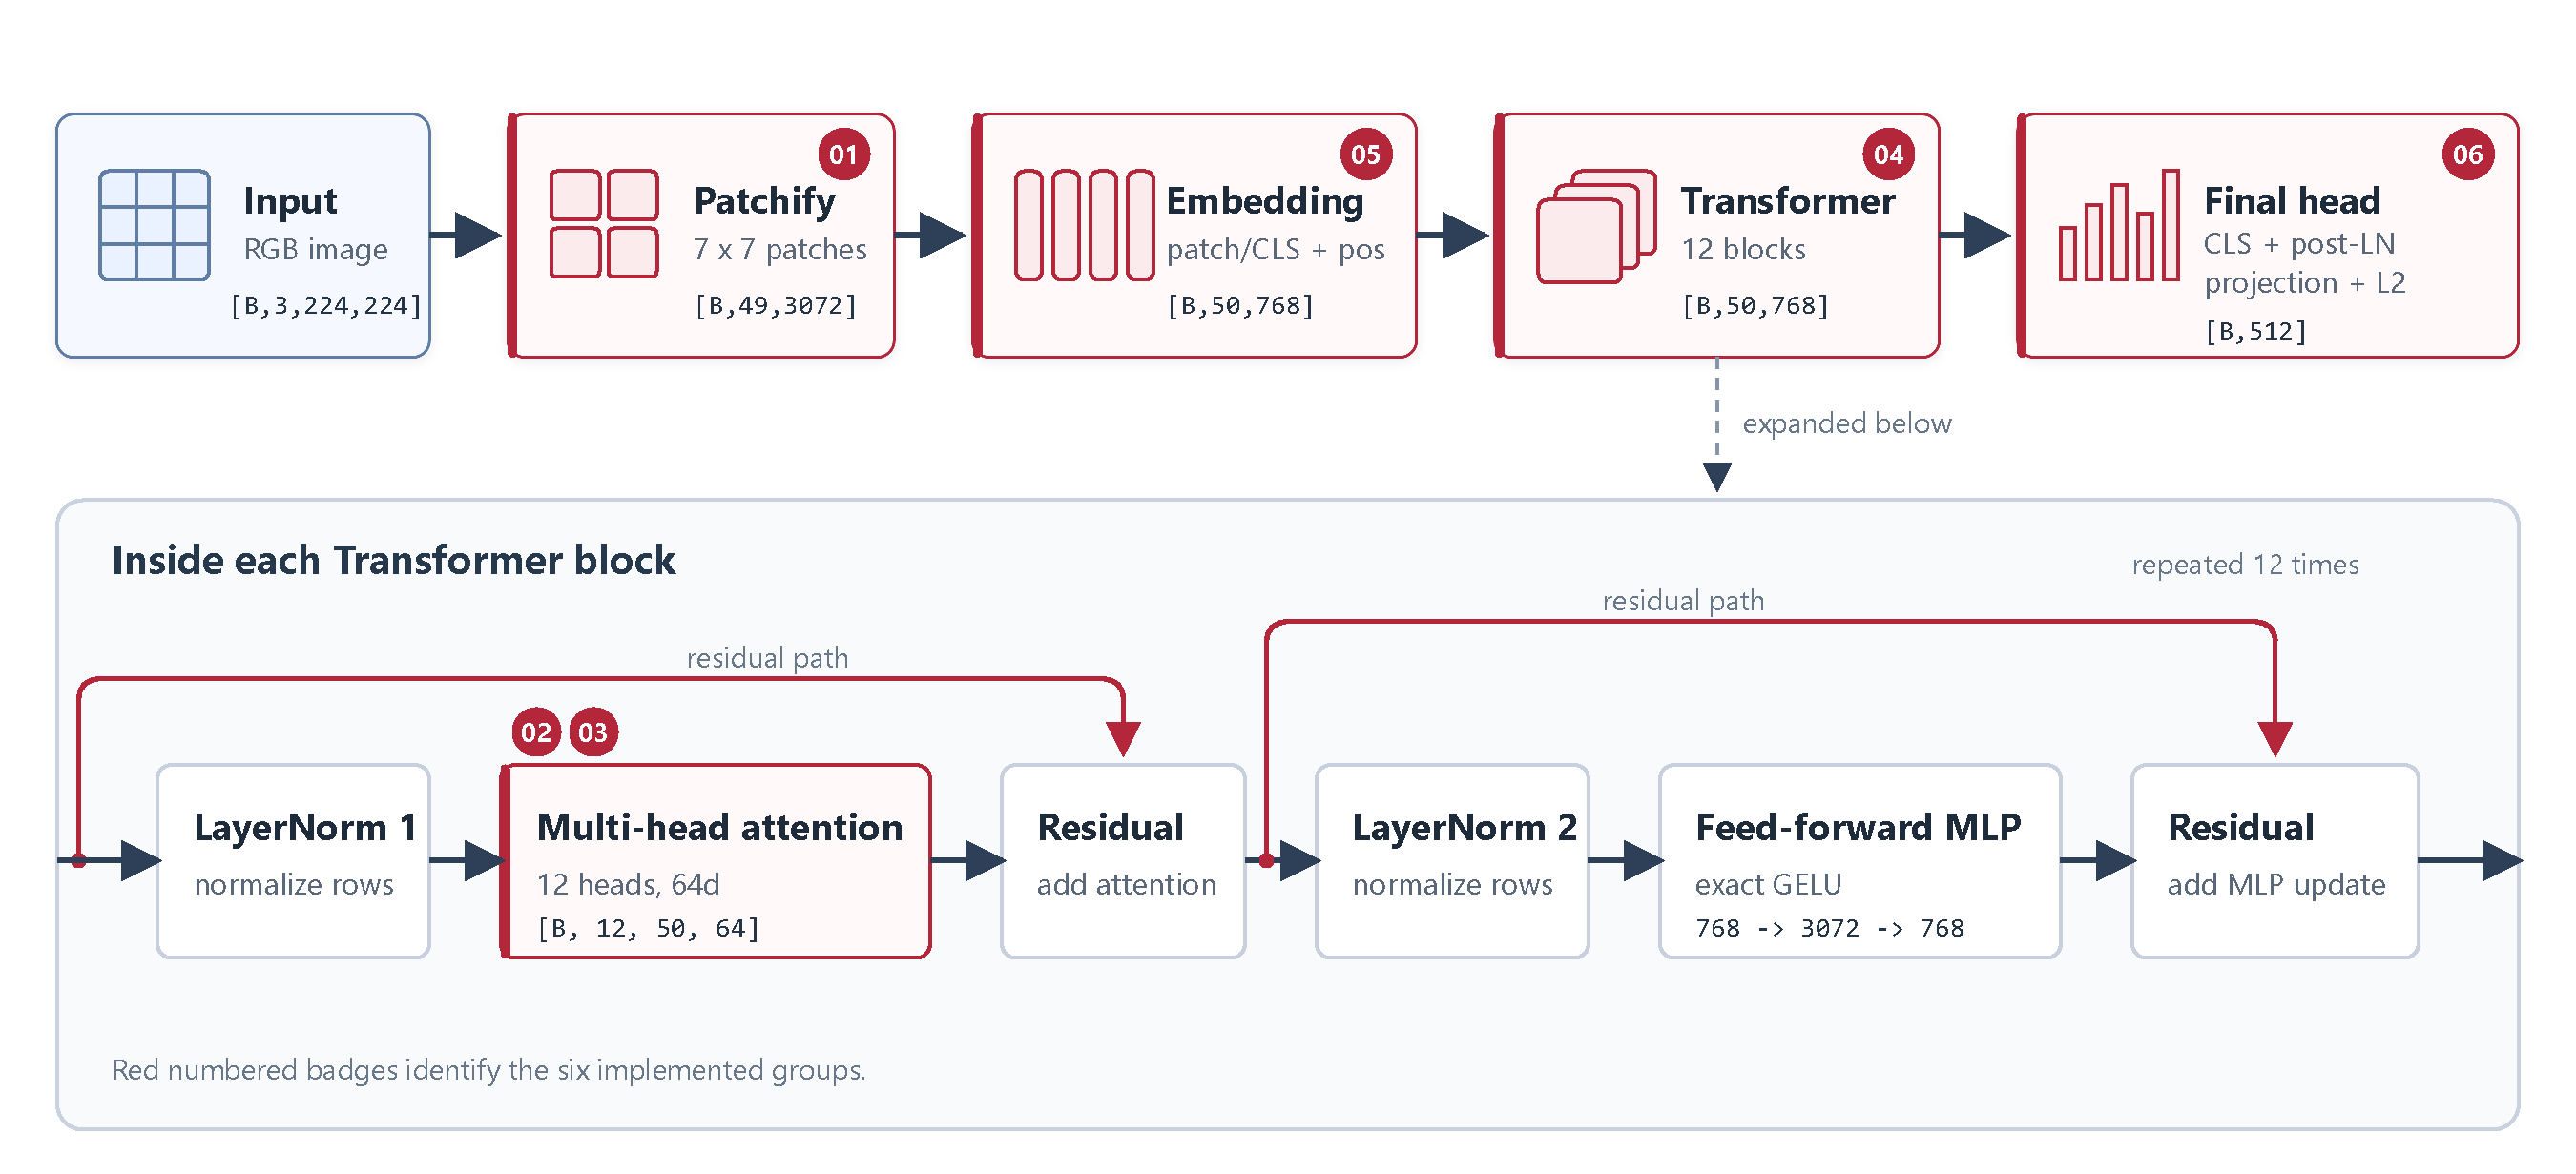
\includegraphics[width=0.98\linewidth]{figs/architecture.pdf}
\caption{OpenCLIP ViT-B/32 image-encoder computation. The upper row follows the
complete data path; the lower panel expands the repeated Transformer block.
Red modules identify the six implementation groups.}
\label{fig:vit-arch}
\end{figure}

\section{Implementations}

All model parameters are loaded from the supplied checkpoint and remain fixed.
The implementation uses NumPy matrix multiplication, reshape, transpose,
broadcasting, and reductions; PyTorch and OpenCLIP are not imported.

\paragraph{TODO-01: Patch extraction.}
The input \([B,3,224,224]\) is reshaped to
\([B,3,7,32,7,32]\), separating the image into a \(7\times7\) patch grid while
retaining each \(32\times32\) RGB patch. Axes are transposed to
\([B,7,7,3,32,32]\), giving row-major patch order and channel-first values
inside every patch. The final reshape produces \([B,49,3072]\). This one
operation changes the representation from a spatial image to a sequence of 49
patch rows.

\paragraph{TODO-02: Splitting attention heads.}
For a token tensor \([B,N,768]\), the feature axis is reshaped to
\(12\times64\) and transposed to \([B,12,N,64]\). The batch and token axes keep
their meanings, while the 12 heads are evaluated independently and the 64
features inside each head remain intact.

\paragraph{TODO-03: Multi-head attention.}
The supplied input projection produces concatenated query, key, and value
tensors. Queries and keys are compared after the head split, scaled by
\(\sqrt{64}=8\), and converted to row coefficients by the supplied stable
attention helper. The coefficients mix the value rows, the head outputs are
transposed back and merged to \([B,N,768]\), and the final attention output is
projected with the stored \([768,768]\) weight.

\paragraph{TODO-04: Transformer block.}
Each block first applies LayerNorm and multi-head attention to the input, then
adds the attention update to the original token tensor. The result is normalized
again before the MLP. The first linear layer expands 768 features to 3072, the
provided exact GELU is applied, and the second linear layer returns to 768
features. A second residual addition forms the block output. This structure is
repeated for all twelve visual Transformer blocks.

\paragraph{TODO-05: Token embedding.}
The supplied convolution weight is reshaped from its stored layout to
\([768,3072]\). Patch rows are projected by matrix multiplication without a
bias. A learned CLS row is repeated over the batch and prepended to the 49
patch rows, producing \([B,50,768]\). The learned \([50,768]\) positional
embedding is then broadcast over the batch and added element by element.

\paragraph{TODO-06: Final image feature.}
After the twelve blocks, row zero is selected as the CLS representation,
reducing \([B,50,768]\) to \([B,768]\). Post-LayerNorm is applied, followed by a
projection from 768 to 512 values. The supplied projection is already stored as
\([768,512]\), so it is not transposed. Each output row is finally divided by
its L2 norm.

\paragraph{Numerical dtype correction.}
The attention scale was initially calculated using the ordinary NumPy square
root of \texttt{head\_dim}:
\[
\texttt{scale = np.sqrt(self.head\_dim)}
\]
NumPy returned a \texttt{float64} scalar, so division promoted the attention
scores to \texttt{float64}; the dtype then propagated through the Transformer
block. \texttt{check.py} reported \texttt{block0: use float32}. Casting the
square root to \texttt{float32} before division preserved the required dtype
throughout the computation.

\section{Results}

The completed implementation was checked with
\texttt{python check.py --stage all}. All eight stages passed. Table~\ref{tab:results}
reports the locally measured maximum and mean absolute errors.

\begin{table}[H]
\centering
\small
\setlength{\tabcolsep}{4pt}
\renewcommand{\arraystretch}{1.05}
\begin{tabular}{@{}lccrr@{}}
\toprule
Stage & Compared shape & Output shape & Max abs. & Mean abs. \\
\midrule
assets & supplied tensors & 152 tensors & -- & -- \\
preprocess & 10 images & \((10,3,224,224)\) & \(0\) & \(0\) \\
patches & 2 images & \((2,49,3072)\) & \(0\) & \(0\) \\
tokens & 2 images & \((2,50,768)\) & \(4.005\times10^{-5}\) & \(1.289\times10^{-6}\) \\
block0 & 2 images & \((2,50,768)\) & \(7.063\times10^{-6}\) & \(3.250\times10^{-7}\) \\
last\_tokens & 2 images & \((2,50,768)\) & \(4.768\times10^{-5}\) & \(2.696\times10^{-6}\) \\
output & 10 images & \((10,512)\) & \(5.439\times10^{-7}\) & \(8.311\times10^{-8}\) \\
batch & 3 images & \((3,512)\) & \(4.619\times10^{-7}\) & \(7.632\times10^{-8}\) \\
\bottomrule
\end{tabular}
\caption{Measured absolute errors for every staged numerical check.}
\label{tab:results}
\end{table}

The final output check is within a maximum absolute error of
\(5.439\times10^{-7}\). The batch check changes image order to
\([1,0,1]\), including a repeated image, and still matches the corresponding
reference rows with maximum absolute error \(4.619\times10^{-7}\). The exported
\texttt{output\_tokens.npz} contains ten IDs, a finite
\texttt{float32} tensor of shape \((10,512)\), and unit-length output rows.

The code and reproduction instructions are available at the
\href{https://github.com/Luo-start/project1-numpy-student}
{project GitHub repository}.

\section{Discussion}

The results show that the NumPy implementation follows the supplied computation
closely at every observable stage. The largest recorded error among the
intermediate checks is \(4.768\times10^{-5}\) for the complete token sequence;
the final unit-normalized 512-dimensional feature remains below
\(5.5\times10^{-7}\). These differences are consistent with the order in which
floating-point matrix products, GELU values, and normalization operations are
evaluated, rather than a mismatch in the model structure.

The dtype problem provides the main implementation lesson. A scalar that
appears harmless can change an entire tensor's precision through NumPy's type
promotion rules. Explicitly constructing the attention scale as
\texttt{float32} keeps the computation chain consistent and avoids silently
converting the Transformer output to \texttt{float64}. The fix is local, but
its effect is global because attention output feeds both residual paths and all
subsequent blocks.

The implementation is intentionally specialized for this fixed checkpoint.
It performs no training or parameter updates, does not include the text tower,
and is not optimized as a high-throughput inference engine. Its purpose is to
make the image-encoder computation explicit and reproducible while retaining
the public interface required by the later multimodal project.

Overall, the objectives are met: the six assessed groups are implemented using
NumPy operations, every staged reference check passes, and the final encoder
returns the required normalized 512-dimensional image features.

\newpage

% ============================================================
% Review and grade page
% ============================================================
\begin{tikzpicture}[remember picture, overlay]
  \draw[thick]
    ($(current page.north west)+(2cm,-3cm)$)
    rectangle
    ($(current page.south east)+(-2cm,3.5cm)$);
\end{tikzpicture}

\vspace{1cm}

\noindent \textbf{指导教师批阅意见：}
\vspace{6cm}
\hfill

\vspace{1cm}

\noindent \textbf{成绩评定：}
\vspace{2cm}
\hfill

\vspace{1cm}

\noindent
\hfill
\textbf{指导教师签字：}\quad\quad\quad\quad\quad\\[0.5cm]

\hfill
\textbf{年}\quad\quad
\textbf{月}\quad\quad
\textbf{日}\quad

\vspace{1cm}

\noindent \textbf{备注：}

\begin{tikzpicture}[remember picture, overlay]
  \node[
    anchor=north west,
    inner sep=0pt,
    text width=\dimexpr\paperwidth-4cm\relax
  ] at ($(current page.south west)+(2cm,3.1cm)$) {
    \begin{minipage}{\dimexpr\paperwidth-4cm\relax}
      \small
      \noindent
      \textbf{注：}\;1、报告内的项目或内容设置，可根据实际情况加以调整和补充。\\[0.2cm]
      \phantom{\textbf{注：}\;}2、教师批改学生实验报告时间应在学生提交实验报告时间后 10 日内。
    \end{minipage}
  };
\end{tikzpicture}

\end{document}
